\documentclass[11pt]{article}
\usepackage[a4paper,margin=1in]{geometry}
\usepackage[T1]{fontenc}
\usepackage{lmodern}
\usepackage{amsmath,amssymb}
\usepackage{booktabs}
\usepackage{graphicx}
\usepackage{caption}
\usepackage{subcaption}
\usepackage{tikz}
\usetikzlibrary{positioning,arrows.meta,calc,fit,backgrounds}
\usepackage[hidelinks]{hyperref}
\usepackage{microtype}
\usepackage{algorithm}
\usepackage{algpseudocode}
\algnotext{EndFunction}\algnotext{EndFor}\algnotext{EndIf}\algnotext{EndWhile}

\captionsetup{font=small,labelfont=bf}
\newcommand{\eml}{\operatorname{eml}}
\newcommand{\E}{\mathrm{E}}
\newcommand{\RATIO}{540}
\newcommand{\NETONE}{3.0}
\newcommand{\NETBATCH}{0.25}
\newcommand{\EMLSEQ}{214}
\newcommand{\EMLWAVE}{4.8}
\newcommand{\EMLBATCH}{3.7}
\newcommand{\NSE}{17.3}
\newcommand{\NSMAC}{0.32}
\newcommand{\WMIN}{1}
\newcommand{\WMAX}{22{,}881}
\newcommand{\WMED}{80}


\title{Reading Handwritten Digits with a Single Binary Operator:\\
Compiling Neural Networks into Pure EML Expressions}
\author{Chanrathnak Borann\thanks{Code and demo: \url{https://github.com/darhnoel/eml-digit-recognition}}}
\date{November 2026}

\begin{document}
\maketitle

\begin{abstract}
Odrzywołek recently showed that the binary operator
$\eml(x,y)=e^{x}-\ln y$, together with the constant~$1$, generates every
function on a scientific calculator~\cite{odrzywolek2026}. A consequence is
that any neural network built from elementary operations can, in principle,
be written as a single expression whose only operator is $\eml$ and whose only
leaves are $1$ and the inputs. We make this concrete. We train a small
multilayer perceptron on MNIST, compile it mechanically into a pure EML
expression, and evaluate that expression on all 10{,}000 test images. The
expression reaches 96.35\% accuracy and agrees with the quantized network on
every test image, with logits that differ by at most $4.3\times10^{-14}$.
The construction is exact but expensive: the expression has 258{,}842
distinct $\eml$ nodes (about $6.8\times10^{8}$ nodes per class score when
fully written out) and depth~152, and it needs more than 500 times the arithmetic per image
of the network it came from. We also
report two numerical limits of EML arithmetic in IEEE double precision. The two parts of the result answer
two different questions. Can an EML expression recognize handwritten digits?
Yes. Can such an expression be learned directly in EML form? Not with current
methods: we obtained it by training an ordinary network and then translating
that network into EML.
\end{abstract}

% ---------------------------------------------------------------------------
\section{Introduction}

Digital logic has a single universal gate: every Boolean function can be
built from NAND alone~\cite{sheffer1913}. Odrzywołek asked whether continuous
mathematics has an analogue and found one by exhaustive search: the operator
\begin{equation}
  \eml(x,y) = e^{x} - \ln y ,
\end{equation}
which, with the constant~$1$, generates the elementary functions of a
scientific calculator, including $+$, $\times$, $\exp$, $\ln$, and the
trigonometric functions~\cite{odrzywolek2026}. Every such expression is a
binary tree generated by the grammar $S \to 1 \mid x \mid \eml(S,S)$.
Because our expressions nest the operator many times, we use the short name
$\E$ from here on: $\E(x,y)$ means exactly $\eml(x,y)=e^{x}-\ln y$.

Feed-forward networks with elementary activations ($\tanh$, the logistic
function, softmax) are themselves elementary functions of their inputs. The
paper therefore notes that conventional networks are special cases of EML
trees~\cite{odrzywolek2026}. That statement is an existence claim. It leaves
open three practical questions, which this note answers for one standard
task:
\begin{enumerate}
  \item \textbf{Construction.} How is an EML expression for a perception task
        actually obtained?
  \item \textbf{Fidelity.} Does the expression still work when evaluated in
        IEEE double precision, where $\ln 0$, overflow and complex branch cuts
        all arise?
  \item \textbf{Cost.} How large, how deep and how expensive is it?
\end{enumerate}

\paragraph{Contributions.}
This note makes four contributions.
\begin{enumerate}
  \item \textbf{A compiler for whole networks.} Compilers already turn
        single formulas into EML trees (Section~\ref{sec:related}); ours
        rewrites an entire trained neural network as one pure EML
        expression. The expression contains only $\E$, the number $1$ and
        the pixel values; even the network's weights are built from $1$
        (Section~\ref{sec:method}).
  \item \textbf{A working demonstration} on two digit datasets,
        MNIST~\cite{lecun1998} and $8\times8$ digits~\cite{alpaydin1998}.
        The EML expressions give exactly the same answers as the networks
        (Section~\ref{sec:results}).
  \item \textbf{Measurements} of how large and how deep the expressions are,
        how much of them can run in parallel, and how long they take to
        compute (Section~\ref{sec:results}).
  \item \textbf{Two limits of EML arithmetic on real computers}, caused by
        the finite range of floating-point numbers
        (Section~\ref{sec:numerics}).
\end{enumerate}

We claim no new expressivity result. The existence of these expressions
follows from~\cite{odrzywolek2026}; the contribution is the explicit
construction, its verification, and its costs.

% ---------------------------------------------------------------------------
\section{Related work}
\label{sec:related}

\paragraph{EML in neural networks.}
Several projects have combined EML with neural networks since the operator
appeared, all keeping ordinary arithmetic somewhere. The \emph{uniop} toolkit
runs a $784\!\to\!32\!\to\!10$ MNIST network whose hidden activation is
$\exp$, that is $\eml(x,1)$, on encrypted inputs; its matrix products remain
ordinary~\cite{uniop}. The \emph{one-op} project ports GPT-2 to ``EML
circuits''; its code keeps standard matrix multiplication, exponentials,
logarithms and square roots~\cite{oneop}. A preprint proposing networks with
an EML tree as the final layer, and dedicated EML hardware, has been
withdrawn by its author~\cite{ipek2026}. Odrzywołek reports that symbolic
regression within an architecture close to standard neural networks remains
beyond reach, and proposes rational ``M\"obius'' layers
instead~\cite{odrzywolek2026b}.

\paragraph{Compiling formulas into EML.}
The original paper includes a compiler from formulas to EML
trees~\cite{odrzywolek2026}. The \emph{eml-sr} and \emph{uniop} projects
provide similar compilers~\cite{emlsr,uniop}; eml-sr has a strict mode in
which the only leaves are $1$ and the variables, as here. These tools work on
individual formulas. To our knowledge, no earlier work compiles a complete
trained classifier into a pure EML expression, with every weight built from
$1$, and checks it on a full test set.

% ---------------------------------------------------------------------------
\section{Background: arithmetic from one operator}
\label{sec:background}

All identities below are from~\cite{odrzywolek2026} or follow directly from
them:
\begin{align}
  e^{x} &= \E(x,1), \\
  \ln x &= \E\bigl(1,\ \E(\E(1,x),1)\bigr), \\
  x - y &= \E(\ln x,\ e^{y}), \label{eq:sub}\\
  0 &= \ln 1, \qquad -y = 0 - y, \qquad x + y = x - (-y), \\
  x \cdot y &= \exp(\ln x + \ln y).
\end{align}
Expanding the inner $\ln$ and $\exp$ in~\eqref{eq:sub} gives the five-node
expression shown in Figure~\ref{fig:recipes}. For negative arguments, $\ln$
is the complex principal branch, so intermediate values can be complex even
when the final result is real; the identities $e^{\ln x}=x$ (for $x\ne0$) and
$\ln e^{y}=y$ (for real $y$) are what make the results come out real.
Table~\ref{tab:recipes} lists the sizes of the forms our compiler uses. They
are not minimal: direct search in~\cite{odrzywolek2026} finds shorter forms
for $x+y$ and $x\cdot y$.

\begin{figure}[htbp]
\centering
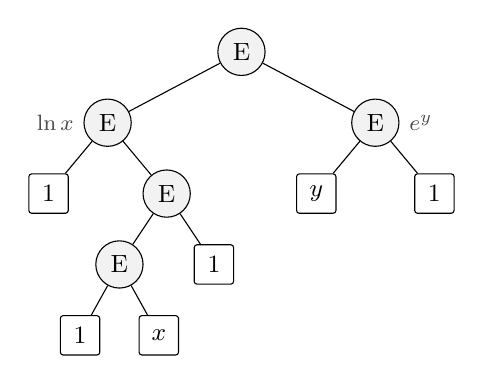
\begin{tikzpicture}[
  every node/.style={font=\small},
  op/.style={circle,draw,minimum size=6mm,inner sep=0pt,fill=black!5},
  leaf/.style={rectangle,draw,rounded corners=1pt,minimum size=5mm,inner sep=1.5pt},
  level distance=9mm,
  level 1/.style={sibling distance=34mm},
  level 2/.style={sibling distance=15mm},
  level 3/.style={sibling distance=12mm},
  level 4/.style={sibling distance=10mm},
  edge from parent/.style={draw,-}]
\node[op] {$\E$}
  child {node[op,label={[font=\footnotesize,text=black!70]left:$\ln x$}] {$\E$}
    child {node[leaf] {$1$}}
    child {node[op] {$\E$}
      child {node[op] {$\E$}
        child {node[leaf] {$1$}}
        child {node[leaf] {$x$}}}
      child {node[leaf] {$1$}}}}
  child {node[op,label={[font=\footnotesize,text=black!70]right:$e^{y}$}] {$\E$}
    child {node[leaf] {$y$}}
    child {node[leaf] {$1$}}};
\end{tikzpicture}
\caption{The subtraction $x-y=\E(\ln x,e^{y})$ written as a pure EML tree.
Every internal node is $\E(a,b)=e^{a}-\ln b$; the leaves are $1$ and the
inputs. The left subtree computes $\ln x$, the right subtree $e^{y}$.}
\label{fig:recipes}
\end{figure}

\begin{table}[htbp]
\centering
\caption{Size of each compiled operation: distinct $\E$ nodes, node count
of the fully written-out tree (including leaves), and depth.}
\label{tab:recipes}
\small
\begin{tabular}{lrrr}
\toprule
Operation & $\E$ nodes & tree nodes & depth \\
\midrule
$e^{x}$       & 1  & 3   & 1 \\
$\ln x$       & 3  & 7   & 3 \\
$x-y$         & 5  & 11  & 4 \\
$x+y$         & 13 & 27  & 9 \\
$x\cdot y$    & 20 & 41  & 10 \\
$\tanh x$     & 35 & 115 & 22 \\
constant $2$  & 9  & 27  & 9 \\
\bottomrule
\end{tabular}
\end{table}

% ---------------------------------------------------------------------------
\section{Method}
\label{sec:method}

Figure~\ref{fig:pipeline} shows the pipeline. Learning happens in one place
only, stage~(b); every later stage is an exact or near-exact rewriting.

\begin{figure*}[t]
\centering
\resizebox{\linewidth}{!}{%
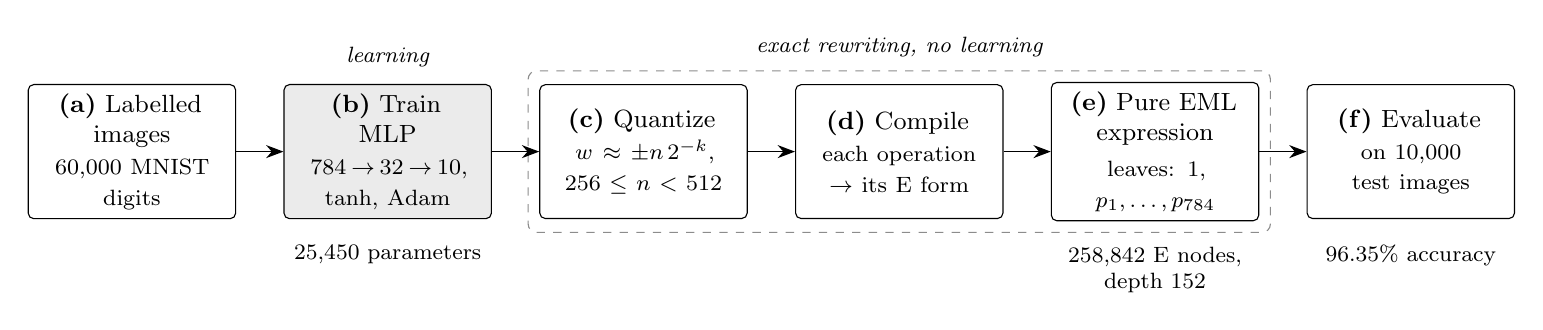
\begin{tikzpicture}[
  font=\small,
  stage/.style={rectangle,draw,rounded corners=2pt,align=center,
                minimum height=17mm,text width=24mm,fill=white},
  learn/.style={stage,fill=black!8},
  arr/.style={-{Stealth[length=2.2mm]},semithick},
  lab/.style={font=\footnotesize\bfseries,anchor=south}]
\node[stage] (data) {\textbf{(a)} Labelled\\images\\[2pt]\footnotesize 60{,}000 MNIST\\ \footnotesize digits};
\node[learn,right=6mm of data] (train) {\textbf{(b)} Train\\MLP\\[2pt]\footnotesize $784\!\to\!32\!\to\!10$,\\ \footnotesize $\tanh$, Adam};
\node[stage,right=6mm of train] (quant) {\textbf{(c)} Quantize\\[2pt]\footnotesize $w\approx\pm n\,2^{-k}$,\\ \footnotesize $256\le n<512$};
\node[stage,right=6mm of quant] (comp) {\textbf{(d)} Compile\\[2pt]\footnotesize each operation\\ \footnotesize $\to$ its $\E$ form};
\node[stage,right=6mm of comp] (expr) {\textbf{(e)} Pure EML\\expression\\[2pt]\footnotesize leaves: $1$, $p_1,\dots,p_{784}$};
\node[stage,right=6mm of expr] (eval) {\textbf{(f)} Evaluate\\[2pt]\footnotesize on 10{,}000\\ \footnotesize test images};
\foreach \a/\b in {data/train,train/quant,quant/comp,comp/expr,expr/eval}
  \draw[arr] (\a) -- (\b);
\node[below=2mm of train,font=\footnotesize,align=center] {25{,}450 parameters};
\node[below=2mm of expr,font=\footnotesize,align=center] {258{,}842 $\E$ nodes,\\depth 152};
\node[below=2mm of eval,font=\footnotesize,align=center] {96.35\% accuracy};
\node[above=1mm of train,font=\footnotesize\itshape] {learning};
\begin{scope}[on background layer]
  \node[draw=black!45,dashed,rounded corners=3pt,inner xsep=4pt,inner ysep=4pt,
        fit=(quant)(comp)(expr)] (grp) {};
\end{scope}
\node[above=0.5mm of grp,font=\footnotesize\itshape] {exact rewriting, no learning};
\end{tikzpicture}}
\caption{From data to a pure EML expression. Only stage (b) learns. Stage (c)
rounds each parameter to a value that can be built from $1$; stage (d)
rewrites every addition, multiplication, $\tanh$ and constant into nested
$\E$ nodes; stage (f) evaluates the expression without any network code.}
\label{fig:pipeline}
\end{figure*}

\subsection{Networks}
For MNIST~\cite{lecun1998} we train a $784\!\to\!32\!\to\!10$ perceptron with
$\tanh$ hidden units, $z=W_2\tanh(W_1x+b_1)+b_2$, using Adam~\cite{kingma2015}
(learning rate $2\times10^{-3}$, batch 128, 15 epochs, weight decay $10^{-5}$).
For the $8\times8$ optical-digits data~\cite{alpaydin1998} (as distributed with
scikit-learn; 1{,}437 training and 360 test images) we train
$64\!\to\!16\!\to\!10$ in the same way. The input scaling (division by 255 or
16) is folded into $W_1$, so the compiled expressions read raw pixel values.
The class is $\arg\max_k z_k$. We compile the ten logits as ten expressions
that share subexpressions; a smooth arg-max is also elementary and could
merge them into one.

\subsection{Constants from 1}
Every leaf is either $1$ or a pixel, so each weight must itself be an
expression in~$1$. We round $|w|$ to $n\,2^{-k}$ with $256\le n<512$
(a 9-bit mantissa, relative error below $2^{-9}$) and build $\ln|w|$ directly:
\[
  \ln|w| = \ln n - k\ln 2 ,
\]
with $n$ and $2$ obtained from~$1$ by repeated doubling and addition, and
$k\ln2$ by doubling $\ln 2$. A product $w\,x$ is then
$\exp(\ln|w| + \ln x)$, entered into a positive or a negative partial sum
according to the sign of $w$. Building constants in the log domain is not
only shorter; it is required, see Section~\ref{sec:numerics}.

\subsection{Compilation and evaluation}
Algorithm~\ref{alg:compile} gives the compiler in full. It has two parts.
The first part (\textsc{Node} to \textsc{Tanh}) is a fixed set of rewrite
rules, one per operation, each built only from $\E$ and $1$ using the
identities of Section~\ref{sec:background}. The second part
(\textsc{CompileMLP}) walks the network layer by layer and applies those
rules. \textsc{Node} never creates the same $\E(a,b)$ twice: if a node with
the same two children exists, it is reused (hash-consing). The result is
therefore a directed acyclic graph in which each distinct subexpression is
stored once; the literal EML tree is the full expansion of this graph.
\textsc{Sum} adds terms in a balanced binary tree, which keeps the depth
logarithmic in the number of terms. Products $w\,x$ are formed as
$\exp(\ln|w|+\ln x)$, and the sign of $w$ decides whether the term enters
the positive or the negative partial sum, so no rule needs a negative
constant.

\begin{algorithm}[!htb]
\caption{Compiling a one-hidden-layer $\tanh$ network into a pure EML
expression. Inputs $W_1\in\mathbb{R}^{H\times D}$, $b_1\in\mathbb{R}^{H}$,
$W_2\in\mathbb{R}^{K\times H}$, $b_2\in\mathbb{R}^{K}$; leaves
$\mathbf{1}$ and $p_1,\dots,p_D$ (the pixels).}
\label{alg:compile}
\small
\begin{algorithmic}[1]
\Statex \textit{Rewrite rules (each returns a node of the graph)}
\Function{Node}{$a,b$} \Comment{the only operator: $\E(a,b)=e^{a}-\ln b$}
  \If{$(a,b)\in\mathcal{T}$} \Return $\mathcal{T}[(a,b)]$ \EndIf
  \State create node $v=\E(a,b)$; \ $\mathcal{T}[(a,b)]\gets v$; \ \Return $v$
\EndFunction
\Function{Exp}{$x$} \Return \textsc{Node}($x,\mathbf{1}$) \EndFunction
\Function{Ln}{$x$} \Return \textsc{Node}($\mathbf{1},\ \textsc{Node}(\textsc{Node}(\mathbf{1},x),\mathbf{1})$) \EndFunction
\Function{Sub}{$x,y$} \Return $\textsc{Node}(\textsc{Ln}(x),\ \textsc{Exp}(y))$ \Comment{$x-y$} \EndFunction
\Function{Add}{$x,y$} \Return \textsc{Sub}($x,\ \textsc{Sub}(\mathbf{0},y)$) \Comment{$\mathbf{0}=\textsc{Ln}(\mathbf{1})$} \EndFunction
\Function{Sum}{$t_1,\dots,t_m$} \Comment{balanced tree of \textsc{Add}; $\mathbf{0}$ if $m=0$}
  \While{more than one term} \State replace each adjacent pair $(t,t')$ by \textsc{Add}($t,t'$) \EndWhile
  \State \Return the remaining term
\EndFunction
\Function{Int}{$n$} \Comment{$1\le n<512$, from $\mathbf{1}$}
  \State $P_0\gets\mathbf{1}$; \ $P_{i}\gets\textsc{Add}(P_{i-1},P_{i-1})$ \Comment{$P_i=2^{i}$}
  \State \Return \textsc{Sum}($P_i$ for each bit $i$ set in $n$)
\EndFunction
\Function{LnConst}{$w$} \Comment{$\ln|w|$, with $|w|$ rounded}
  \State choose $k$ and $256\le n<512$ with $|w|\approx n\,2^{-k}$
  \State $L_k\gets$ \textsc{Sum}($k$ copies of $\textsc{Ln}(\textsc{Int}(2))$), built by doubling
  \State \Return \textsc{Sub}($\textsc{Ln}(\textsc{Int}(n)),\ L_k$) \Comment{use \textsc{Add} if $k<0$}
\EndFunction
\Function{Tanh}{$a$} \Comment{$\tanh a = 1-2/(e^{2a}+1)$}
  \State $d\gets\textsc{Add}(\textsc{Exp}(\textsc{Add}(a,a)),\ \mathbf{1})$
  \State \Return \textsc{Sub}($\mathbf{1},\ \textsc{Exp}(\textsc{Sub}(\textsc{Ln}(\textsc{Int}(2)),\ \textsc{Ln}(d)))$)
\EndFunction
\Function{Affine}{$\ell_1,\dots,\ell_m;\ w_1,\dots,w_m;\ c$} \Comment{$\sum_i w_i x_i + c$, given $\ell_i=\ln x_i$}
  \State $\mathcal{P}\gets[\,]$, \ $\mathcal{N}\gets[\,]$
  \For{$i=1,\dots,m$ with $w_i\neq0$}
    \State $t\gets\textsc{Exp}(\textsc{Add}(\textsc{LnConst}(w_i),\ \ell_i))$ \Comment{$|w_i|\,x_i$}
    \State append $t$ to $\mathcal{P}$ if $w_i>0$, else to $\mathcal{N}$
  \EndFor
  \State append $\textsc{Exp}(\textsc{LnConst}(c))$ to $\mathcal{P}$ or $\mathcal{N}$ by the sign of $c$
  \State \Return \textsc{Sub}($\textsc{Sum}(\mathcal{P}),\ \textsc{Sum}(\mathcal{N})$)
\EndFunction
\Statex
\Statex \textit{The network}
\Function{CompileMLP}{$W_1,b_1,W_2,b_2$}
  \For{$i=1,\dots,D$} $\ell_i\gets\textsc{Ln}(p_i)$ \EndFor
  \For{$j=1,\dots,H$}
    \State $h_j\gets\textsc{Tanh}(\textsc{Affine}(\ell;\ W_1[j,:];\ b_1[j]))$; \ $m_j\gets\textsc{Ln}(h_j)$
  \EndFor
  \For{$k=1,\dots,K$} $r_k\gets\textsc{Affine}(m;\ W_2[k,:];\ b_2[k])$ \EndFor
  \State \Return $r_1,\dots,r_K$ \Comment{class scores; the prediction is $\arg\max_k r_k$}
\EndFunction
\end{algorithmic}
\end{algorithm}

Evaluation computes every node as
$e^{a}-\ln b$ in NumPy \texttt{complex128}, which follows the C99 Annex~G
rules for special values ($\ln 0=-\infty$, $e^{-\infty}=0$)~\cite{c99}. The
nodes at equal depth do not depend on each other, so the graph can be
evaluated level by level, one vectorized operation per level.

\subsection{Numerical limits of EML arithmetic}
\label{sec:numerics}
Two limits appeared in practice.

\emph{Range.} Subtraction~\eqref{eq:sub} evaluates $e^{y}$. In double
precision $e^{y}$ overflows for $y\gtrsim709.8$ and underflows to $0$ for
$y\lesssim-745$, after which $\ln$ returns $\pm\infty$ and the result is
wrong. Building the integer $4096$ by repeated addition fails for exactly this
reason: the intermediate $-2048$ makes $e^{-2048}$ underflow. All values that
enter a subtraction as $y$ must therefore stay well inside this range, which
is why constants are built in the log domain.

\emph{Special values.} The chain $\ln 0 = \E(1,\E(\E(1,0),1))$ must pass
through $+\infty$. In PyTorch~2.15 (CPU, \texttt{complex128}) the complex
subtraction $(e+0i)-(-\infty+0i)$ returns $\infty+\mathrm{NaN}\,i$, and the
NaN then propagates to every zero pixel. NumPy returns $\infty+0i$ and the
chain yields $\ln 0=-\infty$ as intended. We therefore evaluate EML
expressions in NumPy.

% ---------------------------------------------------------------------------
\section{Results}
\label{sec:results}

\subsection{Fidelity and size}
Table~\ref{tab:main} summarizes both compiled classifiers. On every test image
the pure EML expression predicts the same class as the quantized network,
and its logits differ from the network's by at most a few units in the
14th digit. Imaginary parts cancel to below $10^{-14}$. Quantization to a
9-bit mantissa does not change accuracy (on MNIST it changes the net
count of correct test images by two). Figure~\ref{fig:examples} shows predictions of the EML
expression on MNIST test images.

\begin{table}[htbp]
\centering
\caption{Two networks compiled into pure EML expressions (leaves: $1$ and
the raw pixels). ``Tree nodes'' counts one class score fully written out.}
\label{tab:main}
\small
\begin{tabular}{lrr}
\toprule
 & $8\times8$ digits & MNIST $28\times28$ \\
\midrule
Network & $64\!\to\!16\!\to\!10$ & $784\!\to\!32\!\to\!10$ \\
Parameters & 1{,}210 & 25{,}450 \\
Test images & 360 & 10{,}000 \\
\midrule
Accuracy, float network & 98.33\% & 96.33\% \\
Accuracy, quantized network & 98.33\% & 96.35\% \\
Accuracy, \textbf{pure EML expression} & \textbf{98.33\%} & \textbf{96.35\%} \\
Agreement with quantized network & 100\% & 100\% \\
Max.\ logit error & $2.5\times10^{-14}$ & $4.3\times10^{-14}$ \\
Max.\ imaginary part & $3.7\times10^{-15}$ & $7.1\times10^{-15}$ \\
\midrule
Distinct $\E$ nodes & 17{,}613 & 258{,}842 \\
Tree nodes per class score & $2.27\times10^{7}$ & $6.80\times10^{8}$ \\
Depth & 134 & 152 \\
\bottomrule
\end{tabular}
\end{table}

\begin{figure}[htbp]
\centering
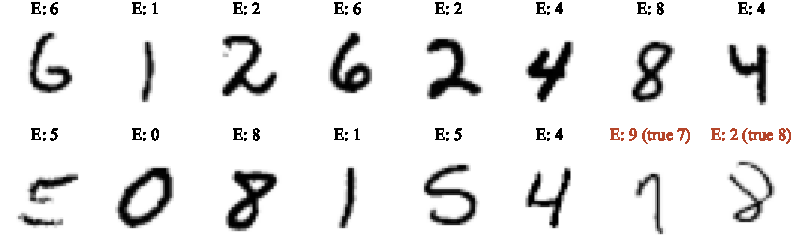
\includegraphics[width=\linewidth]{figures/examples.pdf}
\caption{MNIST test images and the class predicted by the pure EML
expression. The last two are among the 3.65\% it gets wrong.}
\label{fig:examples}
\end{figure}

\subsection{Cost}
The expression replaces each of the network's 25{,}408 multiply--adds with
tens of $\E$ nodes (Table~\ref{tab:recipes}), and each $\E$ node is a complex
exponential and a complex logarithm rather than one fused multiply--add.
Table~\ref{tab:speed} reports measured times on one CPU core. Counting
arithmetic only, the EML form costs about $\RATIO\times$ more per image; the
measured gap is larger because the network runs as dense matrix products,
for which hardware is optimized, while the EML graph does not.

\begin{table}[htbp]
\centering
\caption{Measured cost on MNIST (Apple M5, NumPy~2.5, one process).}
\label{tab:speed}
\small
\begin{tabular}{lr}
\toprule
Network, one image & \NETONE\ $\mu$s \\
Network, per image in a batch of 10{,}000 & \NETBATCH\ $\mu$s \\
EML, one image, node by node & \EMLSEQ\ ms \\
EML, one image, level by level & \EMLWAVE\ ms \\
EML, per image in a batch of 100, level by level & \EMLBATCH\ ms \\
\midrule
One complex $\E$ node & \NSE\ ns \\
One real multiply--add & \NSMAC\ ns \\
Storage: network (float32) / expression (text) & 102\,KB / 6.3\,MB \\
\bottomrule
\end{tabular}
\end{table}

\paragraph{Parallelism.}
The expression can be computed partly in parallel, but only in 152 rounds
that must run one after another, because each round needs results from
earlier ones. Within a round all $\E$ nodes are independent (between
\WMIN\ and \WMAX\ per round), and computing round by round instead of node by
node reduces the time for one image from \EMLSEQ\,ms to \EMLWAVE\,ms; the
network needs only two such rounds, its two layers.

\subsection{Real images}
The expressions read pixel values in the format of their training data. We
convert arbitrary photographs to the MNIST format with the procedure used to
build MNIST: threshold the ink, crop, scale the longer side to 20 pixels with
anti-aliasing, and centre the centre of mass in a $28\times28$ frame. As a
check, 1{,}000 MNIST test digits were enlarged ten times, placed off-centre
on a light background with Gaussian noise ($\sigma=8$), and converted back:
the EML expression classified 96.5\% correctly, against 96.3\% on the
original pixels of the same images. Printed digits in a sans-serif font were
read correctly 7 times out of 10. The errors fall on glyphs whose printed
shape differs from handwriting ($1$, $6$, $9$), which reflects the training
data, not the EML form.

% ---------------------------------------------------------------------------
\section{Discussion}

\paragraph{Expressing versus learning.}
The experiments separate two properties. EML \emph{expresses} digit
recognition: an expression with only $\E$, $1$ and pixels reads handwritten
digits as accurately as the network it came from. EML does not by itself
\emph{learn} it: the expression has no numeric parameters to adjust, only a
shape, and a shape of depth 152 is far beyond the depths at which EML trees
can currently be found by optimization: recovery from random starts falls
from 100\% at depth~2 to under 1\% at depth~5~\cite{odrzywolek2026}.
Odrzywołek also reports that learning EML expressions inside network-like
architectures remains beyond reach~\cite{odrzywolek2026b}, and an independent
study found that EML layers train worse than ReLU and Kolmogorov--Arnold
layers, because of the exploding gradient of the $\ln$
branch~\cite{emlablation}. The working route is to learn with a
parametric model and then compile. The analogy with NAND is close: every
digital OCR program is, at the gate level, a NAND circuit, yet such circuits
are compiled from programs and are not searched for gate by gate.

\paragraph{Size.}
A rough information argument says no tiny EML expression can do this task: a
tree whose leaves are only $1$ and the inputs encodes its knowledge in its
shape, and a digit classifier needs thousands of learned quantities. Our
compiled expressions are, however, far from minimal; for example
Table~\ref{tab:recipes} uses 13 nodes for $x+y$, and the paper's direct search
finds 9. How small an EML expression for MNIST can be is open. The compiled
expression is a natural starting point for such a search, since the paper
reports that optimization recovers EML trees reliably when started near a
solution, even at depths where random starts fail.

\paragraph{Hardware.}
On processors built around multiply--add, the EML form is slower by orders of
magnitude. Its one structural advantage is uniformity: a single operation
repeated. Bipolar transistors compute exponentials and logarithms natively,
which is the basis of translinear circuits~\cite{gilbert1975}, and
Odrzywołek suggests EML as a building block for analog
computing~\cite{odrzywolek2026}. The eml-sr project simulates analog EML
cells, including a translinear design, to measure how component noise
accumulates with tree depth~\cite{emlsr}. An expression of depth~152, like
ours, would be a demanding case for such hardware, and its complex
intermediate values a further obstacle. We have not studied this
ourselves.

\paragraph{Limitations.}
We compiled two small networks on two digit datasets; larger or
convolutional networks compile the same way but have not been measured.
Timing results depend on the implementation and hardware.

% ---------------------------------------------------------------------------
\section{Conclusion}
A handwritten-digit classifier can be written as a single expression in the
operator $e^{x}-\ln y$ and the constant $1$, and that expression works in
ordinary double precision: 96.35\% on MNIST, identical to its source network
on all 10{,}000 test images. It is obtained by compiling a trained network;
it is about ten times larger than the network in distinct operations and
thousands of times slower to evaluate on a CPU. Whether much smaller EML expressions for
such tasks exist, and whether they can be found, are the open questions this
leaves.



\begin{thebibliography}{99}\small
\bibitem{odrzywolek2026}
A.~Odrzywołek.
\newblock All elementary functions from a single operator.
\newblock arXiv:2603.21852, 2026.

\bibitem{sheffer1913}
H.~M. Sheffer.
\newblock A set of five independent postulates for Boolean algebras, with
  application to logical constants.
\newblock \emph{Trans.\ Amer.\ Math.\ Soc.}, 14(4):481--488, 1913.

\bibitem{lecun1998}
Y.~LeCun, L.~Bottou, Y.~Bengio, and P.~Haffner.
\newblock Gradient-based learning applied to document recognition.
\newblock \emph{Proc.\ IEEE}, 86(11):2278--2324, 1998.

\bibitem{alpaydin1998}
E.~Alpaydin and C.~Kaynak.
\newblock Optical recognition of handwritten digits.
\newblock UCI Machine Learning Repository, 1998.

\bibitem{kingma2015}
D.~P. Kingma and J.~Ba.
\newblock Adam: A method for stochastic optimization.
\newblock In \emph{ICLR}, 2015.

\bibitem{c99}
ISO/IEC 9899:1999.
\newblock Programming languages -- C, Annex G: IEC 60559-compatible complex
  arithmetic.

\bibitem{gilbert1975}
B.~Gilbert.
\newblock Translinear circuits: a proposed classification.
\newblock \emph{Electronics Letters}, 11(1):14--16, 1975.

\bibitem{odrzywolek2026b}
A.~Odrzywołek.
\newblock Diversity of EML-type operators.
\newblock arXiv:2609.11210, 2026.

\bibitem{ipek2026}
E.~Ipek.
\newblock Hardware-efficient neuro-symbolic networks with the Exp-Minus-Log
  operator.
\newblock arXiv:2604.13871, 2026 (withdrawn).

\bibitem{uniop}
uniop: a symbolic-regression, compilation, and emission toolkit over a single
  binary operator.
\newblock \url{https://github.com/vmallela0/uniop}, 2026.

\bibitem{oneop}
one-op: continuous Sheffer primitives for deep learning.
\newblock \url{https://github.com/atveit/one-op}, 2026.

\bibitem{emlsr}
eml-sr: EML symbolic regression, compiler and analog noise simulations.
\newblock \url{https://github.com/oaustegard/eml-sr}, 2026.

\bibitem{emlablation}
EML: Exp-Minus-Log neural networks, an ablation study.
\newblock \url{https://github.com/SebastienSeg/eml-ablation-}, 2026.
\end{thebibliography}


\end{document}
